\documentclass{sigchi}

% Use this command to override the default ACM copyright statement (e.g. for preprints). 
% Consult the conference website for the camera-ready copyright statement.


%% EXAMPLE BEGIN -- HOW TO OVERRIDE THE DEFAULT COPYRIGHT STRIP -- (July 22, 2013 - Paul Baumann)
\toappear{Permission to make digital or hard copies of all or part of this work for personal or classroom use is 	granted without fee provided that copies are not made or distributed for profit or commercial advantage and that copies bear this notice and the full citation on the first page. Copyrights for components of this work owned by others than ACM must be honored. Abstracting with credit is permitted. To copy otherwise, or republish, to post on servers or to redistribute to lists, requires prior specific permission and/or a fee. Request permissions from permissions@acm.org. \\
{\emph{CHI'14}}, April 26--May 1, 2014, Toronto, Canada. \\
Copyright \copyright~2014 ACM ISBN/14/04...\$15.00. \\
DOI string from ACM form confirmation}
%% EXAMPLE END -- HOW TO OVERRIDE THE DEFAULT COPYRIGHT STRIP -- (July 22, 2013 - Paul Baumann)


% Arabic page numbers for submission. 
% Remove this line to eliminate page numbers for the camera ready copy
\pagenumbering{arabic}


% Load basic packages
\usepackage{balance}  % to better equalize the last page
\usepackage{graphics} % for EPS, load graphicx instead
\usepackage{times}    % comment if you want LaTeX's default font
\usepackage{url}      % llt: nicely formatted URLs
% use subfig
\usepackage{caption}
\usepackage{subcaption}


% llt: Define a global style for URLs, rather that the default one
\makeatletter
\def\url@leostyle{%
  \@ifundefined{selectfont}{\def\UrlFont{\sf}}{\def\UrlFont{\small\bf\ttfamily}}}
\makeatother
\urlstyle{leo}


% To make various LaTeX processors do the right thing with page size.
\def\pprw{8.5in}
\def\pprh{11in}
\special{papersize=\pprw,\pprh}
\setlength{\paperwidth}{\pprw}
\setlength{\paperheight}{\pprh}
\setlength{\pdfpagewidth}{\pprw}
\setlength{\pdfpageheight}{\pprh}

% Make sure hyperref comes last of your loaded packages, 
% to give it a fighting chance of not being over-written, 
% since its job is to redefine many LaTeX commands.
\usepackage[pdftex]{hyperref}
\hypersetup{
pdftitle={Visually Impaired Users on an online Social Network},
pdfauthor={LaTeX},
pdfkeywords={SIGCHI, proceedings, archival format},
bookmarksnumbered,
pdfstartview={FitH},
colorlinks,
citecolor=black,
filecolor=black,
linkcolor=black,
urlcolor=black,
breaklinks=true,
}

% create a shortcut to typeset table headings
\newcommand\tabhead[1]{\small\textbf{#1}}


% End of preamble. Here it comes the document.
\begin{document}

\title{Activities, Content, and Network Structure of Visually Impaired Users on an Online Social Network}

\numberofauthors{3}
\author{
  \alignauthor 1st Author Name\\
    \affaddr{Affiliation}\\
    \affaddr{Address}\\
    \email{e-mail address}\\
    \affaddr{Optional phone number}
  \alignauthor 2nd Author Name\\
    \affaddr{Affiliation}\\
    \affaddr{Address}\\
    \email{e-mail address}\\
    \affaddr{Optional phone number}    
  \alignauthor 3rd Author Name\\
    \affaddr{Affiliation}\\
    \affaddr{Address}\\
    \email{e-mail address}\\
    \affaddr{Optional phone number}
}

\maketitle

\begin{abstract}


In this paper we present the first large-scale empirical study of how visually impaired people use online social networks, specifically Facebook. We identify a sample of 50K visually impaired users, and study the activities they perform, the content they produce, and the friendship networks they build on Facebook. We find that visually impaired users participate on Facebook (e.g. status updates, comments, likes) as much as the general population, and receive more feedback (i.e., comments and likes) on average on their content. By analyzing the content produced by visually impaired users, we find that they share their experience and issues related to vision impairment. We also identify distinctive patterns in their language and technology use. We also show that, compared to other users, visually impaired users have  smaller social networks, but such differences have decreased over time. Our findings have implications for improving the utility and usability of online social networks for visually impaired users, and can shed light on the design of more accessible sociotechnical systems.




\end{abstract}

\keywords{
	visually impaired users; vision disability; social media; social networking sites; Facebook;
}

\category{H.5.m.}{Human Factors}{Measurement}

\section{Introduction}
Vision-impairement is a prevalent health problem worldwide:  recent statistics \cite{who_report, facts_about_blindness} show that there are 285 million visually impaired people globally and 6.6 million in the US. However, there is a lack of research work of visually impaired users on the Internet, primarily due to the lack of systematic methods to identify this particular population. Among the few existing works on blind users and the Internet, most focus on usability testing for improving the accessibility of specific  online services or applications, with results collected through survey and/or in-person interviews \cite{wentz2011, jayant2011, brady2013cscw, brady2013chi}.  As a result, we only have a rudimentary understanding of how visually impaired people use the Internet today. 

This paper is the first attempt to answer this question quantatively with big data, with special interest placed on how visually impaired users engage with online social networks, in this case Facebook.


The prevelance of social networking services has grown rapidly in  recent years. Since one of the most crucial utilities of the Internet is to access information and most online social networks (e.g. Facebook, Twitter) have been intentionally designed to assist the flow of information through them, it is not surprising that online social networks have become a major part of many people's online experience. For example,  $69\%$ of American Internet users are also Facebook users, and the average time they spend on social networking sites has almost tripled since 2006, accounting for $18\%$ of the total time spent online \cite{facebook_wiki,facebook_stat_wiki,sociallyaware}.

Visually impaired people engage with online social networking sites just as everyone else does. With technologies such as screen reader software, OCR readers, and the Web Accessibility Initiative - Accessible Rich Internet Applications (WAI-ARIA) standard \cite{wai-aria}, visually impaired users can navigate social networking sites through desktop computers or mobile devices~\cite{wentz2011}.  In a recent study of 191 blind people recruited online, $92\%$ of the respondents reported using at least one social networking site, and $80\%$ of them use Facebook \cite{brady2013cscw}.  Despite the high penetration rate of Facebook among visually impaired people, our knowledge about how they engage with Facebook is very limited. There are many basic questions to be answered. What do they do on Facebook? What content do they share? Who do they interact with? What do their social networks look like? 

%For example, Facebook has over $1.15$ billion users in total, covering over $69\%$ of all Internet users in North America and $67\%$ in Middle-East-Africa . 
 
%One of the crucial part of Internet is to gain access to information, which exactly align with the major utility for online social networks such as Facebook and Twitter are specially optimized for.

%Technologies that enable blind users to access the web. The usage of online social networks among blind users. Ratio of adoption for Facebook and Twitter, and also the why that Facebook resembles more a personal friendship network whereas Twitter as a news channel - justify why only studying Facebook. 

In this paper, we present insights about the use of Facebook by 50K visually impaired users in several perspectives, including their Facebook activities, the content they produce, and the structural characteristics of their friendship networks. Our study is motivated by the following research questions.

\emph{RQ1: does the behavior pattern of visually impaired users significantly differ from the pattern of other users?}
 
There are many barriers that may prevent visually impaired users from fully engaging with Facebook. Technologically, the use of  JavaScript to create highly dynamic web pages can cause problems for screen readers, and bugs related to accessibility can be harder to capture and reproduce. Practically, certain Facebook features, such as photo sharing, seem tailored to sighted users. These make up some of the most popular features on Facebook.  

On the other hand, the advancement of assistive technologies such as screen readers and voice input may have  already overcome many barriers, enabling visually impaired users to use the site as easily as anyone. For example, user studies have found that visually impaired users can complete most tasks with increasing ease through Facebook's mobile interface \cite{wentz2011}. And there are also several new photography applications that help visually impaired users take photos and identify objects from the photos taken \cite{jayant2011, taptapsee}. In fact, one of the most famous users on Instagram, Tommy Edison\footnote{\url{http://instagram.com/blindfilmcritic}}, is blind since birth and has uploaded over 300 photos to tens of thousands of followers.

%One`s intuition can be that given all sorts of accessibility issues reported by users\footnote{Facebook Accessibility: \url{https://www.facebook.com/accessibility}} or in the literature \cite{wentz2011}, visually impaired users may find it difficult to fully engage with online SNS as the sighted users do.

%On the other hand, the devolopment of assistive technologies such as screen reader and voice input may have  already broke the barrier, enabling blind users to use the site as easily as for the sighted.

%One good example is photography applications that targeted at the blind populations.
If visually impaired users' ability to engage with Facebook is not constrained by physical difficulties, do they interact with friends on Facebook the same way others do? In some sense, they are a minority group, and they may have special concerns about exposing themselves in a virtual environment. For example, a recent qualitative study showed that blind users feel more uncomfortable asking vision-related questions on Facebook than offline, due to a combination of low response rates and the concern about appearing to be overly dependent to their Facebook friends~\cite{brady2013cscw}. Indeed, it is not clear how other users perceive and interact with visually impaired users on Facebook. 

Are they aware of, or sensitive to the existence of visually impaired users around them? If they do, do they behave differently  around these users? For example, when a visually impaired user shares a photo, do his/her friends feel more inspired or obligated to respond to, comparing to a photo shared by another friend? 

This work is to show the difference between the feedback received by visually impaired users and the average users, and if there is any, explore the motif of such difference. 

How can interprete the feedback they received from other users? How they think of Facebook, as a support group?

\emph{RQ2: when visually impaired users engage with social networking sites, what kind of content do they produce and share? }

Cite research of VizWiz
Previous research has shown that the visually impaired users while are able to leverage social networks to .., but are hestiate to do because of the 

In addition to that, people with cognitive disabilities, such as autism, have privacy concerns when talkng about their conditions online~\cite{burke:2010}. However, engaging with online social networks has also been found to be generally positive and beneficial for people with disabilities or medical conditions \cite{burke:2010,tsaousides2011}. Taken together, minority groups on online social networks have to decide how much to share about their conditions to gain social support without paying a high social cost. Are visually impaired users on Facebook facing the same dilemma?  Do they share their problems and issues, or do they prefer more general topics, keeping their visual challenges behind their computer screens? When engaging with large, general-purpose social networks like Facebook, both behaviors seem reasonable. By analyzing the textual content of visually impaired users' status updates and photo captions, we will offer insights on the overall trend at a high level.


\emph{RQ3: how are visually impaired users' social networks structured? }

Previous research suggested that blind users have smaller and denser social networks \cite{brady2013cscw}, but this result is obtained from survey response by a small group of blind people. To what extent is this true for visually impaired users at a large scale on Facebook? Also, as homophily theory would predict that people with vision impairement are more likely to be friends with each other, can we quantitatively verify the effect of homophily here? If the homophily effect is significant and visually impaired users are well-connected to communities of people with vision impairment, would that expand their social networks beyond their offline social circles, thus situate them in larger social networks? 


Answers to these questions will not only offer us a broader view on how  visually impaired people engage in online social networks, but also lead to the development of more general and accurate methods for identifying visually impaired users online. 

Some websites or products create an enhanced experience for visually impaired users.


\section{Related Work}

The value of online social networks has been widely acknowledged. By connecting people and propagating    information among them, online social networks are able to foster communities \cite{backstrom2006}, spread new opinions and behaviors~\cite{romero2011,wu2011}, deliver critical information rapidly in reaction to crisis \cite{Goolsby:2010}, and even lead to societal changes \cite{weber2013}.  For individuals, the value of online social networks varies across social groups. Many previous studies looked at how different social groups engage with online social networks. boyd et al. \cite{boyd2007} studied the use of online social networks by teenagers and young adults, claiming that social networks are crucial for young adults to ``work out identity and status, make sense of cultural cues, and negotiate public life'. As shown a study by Pew Research Center, $43\%$ of American Internet users older than 65 are using online social networks today (mostly, Facebook), and the major functions of social media for seniors is to maintain ties with family, particularly those who live far way \cite{pew_seniors}. Burke et al studied how families communicate on Facebook, showing distinctive patterns in the way parents talk to their children compared to talk to their friends~\cite{burke2013}.  Very recently, Morris et al focused their study on how new mothers use social media, and found signficant changes in new mothers' behaviorial patterns (e.g., site choice, post content, post frequency) pre and after child-birth~\cite{morris2014}. The general theme found in these works is that people of different social groups are adopting and embracing online social networks for distinct reasons, which inform the ways in which these different social groups interact with social media. 

%although many of them have various levels of privacy concerns, and the way of interacting with social media can be very characteristic for a given social group.

Among this large body of research on social media usage by specific social groups, there has been relatively few studies on people with disabilities. Burke et al~\cite{burke:2010} looked how people with autism use social media, and found that although the online communications can be less stressful and more supportive, autism patients find it difficult to maintain online connections and trust online ``friends''. Tsaousides et al~\cite{tsaousides2011} surveyed individuals with traumatic brain injury, finding that most of them either already use Facebook regularly or have great interests at learning to use Facebook. However, their further engagement with Facebook is hindered by security concerns and cognitive deficits. Indeed, comparing to other social groups, people with disabilities need to overcome substantial technological and cognitive barriers to fully engage with online social networks. 

Most existing work studying visually impaired people on online social networks has emphasized on assessing and removing these barriers. Wentz et al~\cite{wentz2011} evaluated the accessibility of Facebook with different interfaces by running usability studies of 15 blind people. They found that   the mobile interface of Facebook is more accessible than the desktop version. In addition, their study demonstrated the popularity of mobile technology (especially smart phones) among blind people.   Bigham et al~\cite{bigham2010} designed \emph{VizWiz}, an iPhone  Q\&A application that allows blind people to take a photo, record a question related to the photos in audio form, and submit the question (both photo and audio) to Amazon Mechanical Turk for answers. Some recent work~\cite{brady2013chi, brady2013cscw} evaluated the use of VizWiz by a few thousand blind users over a year, categorized the questions they asked, and explored the appropriateness of leveraging online social networks as friendsourced Q\&A platforms for blind people. Their results are in consistency with previous findings~\cite{burke:2010,tsaousides2011}: while online social networks can potentially provide tremendous support to people with disabilities, the social costs of exposing one's problems and vulnerability is a serious concern for these users. 

Although developed along this line of research, our work differs from previous studies in two ways: first, we study  the general patterns of how visually impaired users engage with Facebook (the largest study of its kind);  second, we investigate several novel perspectives of visually impaired users' activities, for example, the textual content they generated, the interaction they perform with friends, and the structural properties of their social networks. 


%The use of online social networks by visually impaired people is an interesting new research topic. Most existing work can be categorized into two areas: 1) evaluating the usability of existing online services; 2) designing new assitive applications on top of social networking sites. 


%To help blind people take better pictures, Jayant et al~\cite{jayant2011} built \emph{EasySnap}, an iPhone application that gives blind users real-time feedback when they take pictures, by detecting human faces and static objects in the view and directing the users to move camera closer to these objects.

%There have been some recent efforts to study people with disabilities on online social networks, many of them highlighted the value of online social networks to people with disabilities \cite{burke:2010,cavender:2010,hong:2012}.

%Parents of kids with special needs turned to social media for informatin, new ideas, and social support.

%http://www.sheknows.com/parenting/articles/1009023/social-media-help-for-parents-of-kids-with-special-needs


%Meanwhile, social networking technologies are getting more and more prevalent among visually impaired people. Although there are some social networking sites specially targeted to blind and visually impaired people (e.g, Inclusive Planet \footnote{\url{www.inclusiveplanet.com}}, Zone BBS \footnote{\url{zonebbs.com}}),  many visually impaired people also use the popular social networking services such as Facebook and Twitter. In fact, a recent study surveying 191 blind people found that $80\%$ and $52\%$ of them participate on Facebook and Twitter, respectively. 

%There has been work evaluating the usability of social networking sites to the blind community. For example,
%\cite{wentz2011} demonstrates the popularity of mobile technology, especially smart phonts, among blind population, showing that mobile apps are more accessible than desktop apps.

%With technology, blind users can take and share photos, too.
%\cite{jayant2011, brady2013chi} present recent research efforts on blind photography. There are also some famous blind social media users such as \textit{blindfilmcritics} on Instagram.

%However, there are some subtlies when visually impaired use social networking sites. 
%For example, they have to consider the tradeoff between getting support and exposing their vulnenability.
%\cite{brady2013cscw} discusses the usefulness of social network as a resource for blind users.

%There has been great work on making Facebook accessible for everyone\footnote{\url{https://www.facebook.com/blog/blog.php?post=71852922130}}.


\section{Data}
%Difficulty with identifying a large population of visually impaired users online.

Equipped with free screen reader software and  a variety of assistive applications\footnote{For example, TapTapSee (\url{http://www.taptapseeapp.com/}), VizWiz \cite{jayant2011}.}, the Apple iPhone has become one of the most popular devices among blind users \cite{brady2013chi}.  Placing strong design emphasis on accessibility from the beginning, Facebook's mobile interface has been known for being more accessible and usable for blind users than the desktop version\cite{wentz2011}.   We therefore focus our study on users who access Facebook on their iPhones through Apple's default screen reader service (VoiceOver). To do so, we detect a visually impaired user if he or she accesses Facebook in VoiceOver mode for at least 3 days in a month\footnote{We filter out people who turned on VoiceOver once or twice, in case they enter VoiceOver mode accidentally.}.  

We first find all Facebook users who accessed Facebook from their iPhone in the period between June 15, 2013 and July 15, 2013. Among them, we draw a random sample of 50K visually impaired users,  and a random sample of 160K users who were active for at least 3 days in this period as the control group. In the rest of this paper, we will refer to the first sample as \textit{VoiceOver sample}, and the second sample as \textit{iOS sample}.


\section{Demographics}
Although our study is limited to the popualation of iPhone users, given the large number of users we sampled, our sample consists of a demographically diverse group of visually impaired users. In this section, we will present the country, age, and gender distribution of visually impaired users in our sample, and compare them with the control group of randomly-sampled iPhone users. All the demographic dimensions we study are based on the self-reported data in user profile pages.

\textbf{Country} We first look at how our sampled users are geographically distributed. Table~\ref{tab:demographics_country} shows the top 5 countries for each group, as reported in user's profile. First thing we notice is that both populations are highly concentrated in developed countries, especially, the United States (with around one third of the users in both samples). Secondly, it is interesting to notice that the iPhone and VoiceOver seem to be more prevalent among vision-impaired users in Europe and America than Asia -- Japan has the 3rd most iPhone users in the general iOS sample, but only ranks at the 14th in the VoiceOver sample. Overall, although our sample of vision-imparied users are highly skewed towards people from developed western countries, it still achieves orders of magnitude more geographical diversity than previous studies, containing users from 183 different countries.

\begin{table}
  \centering
  \begin{tabular}{|c|c|c|}
    \hline
    \tabhead{Rank} &
      VoiceOver sample & iOS sample \\
%    \multicolumn{1}{|p{0.3\columnwidth}|}{\centering\tabhead{Caption --- pre-2002}} &
 %   \multicolumn{1}{|p{0.4\columnwidth}|}{\centering\tabhead{Caption --- 2003 and afterwards}} \\
    \hline
    1 & US ($32.5\%$) & US ($35.5\%$) \\
    \hline
    2 & UK ($7.2\%$) &  UK ($7.3\%$)\\
    \hline
   3 & France ($4.9\%$) & Japan ($4.9\%$) \\
    \hline 
   4 & Gemany ($4.3\%$) & Canada ($3.8\%$)\\
   \hline
   5 & Italy ($4.1\%$) & Germany ($3.6\%$)\\
   \hline
  \end{tabular}
  \caption{Top 5 self-reported countries for users in VoiceOver sample and iOS sample, with their percentages in each sample. }
  \label{tab:demographics_country}
\end{table}

\textbf{Age}  Not surprisingly, both samples are skewed towards young adults, with over $50\%$ of the people in their 20s and 30s, slightly less than one quarter of the sample in their teens, and around one quarter above 40 years old. There are only a few people in our sample who do not report their ages, and we also filter out people who self-report as being over 90 years old. The average age for the VoiceOver sample is 30.14 years old, and for iOS sample is 30.43 years old. We do not see significant difference in terms of age distribution between the visually impaired user group and the control group.

\textbf{Gender} Both genders are well represented in two samples. However, there are slightly more males ($51.8\%$) than females ($47.6\%$) in the VoiceOver sample, but more females ($51.9\%$) than males in the iOS sample ($47.1\%$).

Note that although the visually impaired users in our sample are much more diverse than previous studies in this field \cite{wentz2011,brady2013chi,brady2013cscw}, it is not a fair representation of the global visually impaired population. By constraining our study to iPhone users on Facebook,  we over-sample users from well-devoloped western countries, who are also younger and with relatively high income. Reaching out to visually impaired population who are under-privileged and unequipped with technologies and understanding their needs is definitely an important issue, but it is out of the scope of this paper due to data and technical limitations.

%To better understand the diversity or limitation 

%Country, age, gender, facebook age, engagement level.

\section{Facebook Activity}


\begin{figure*}[t]
\centering
\begin{subfigure}[b]{0.22\textwidth}
    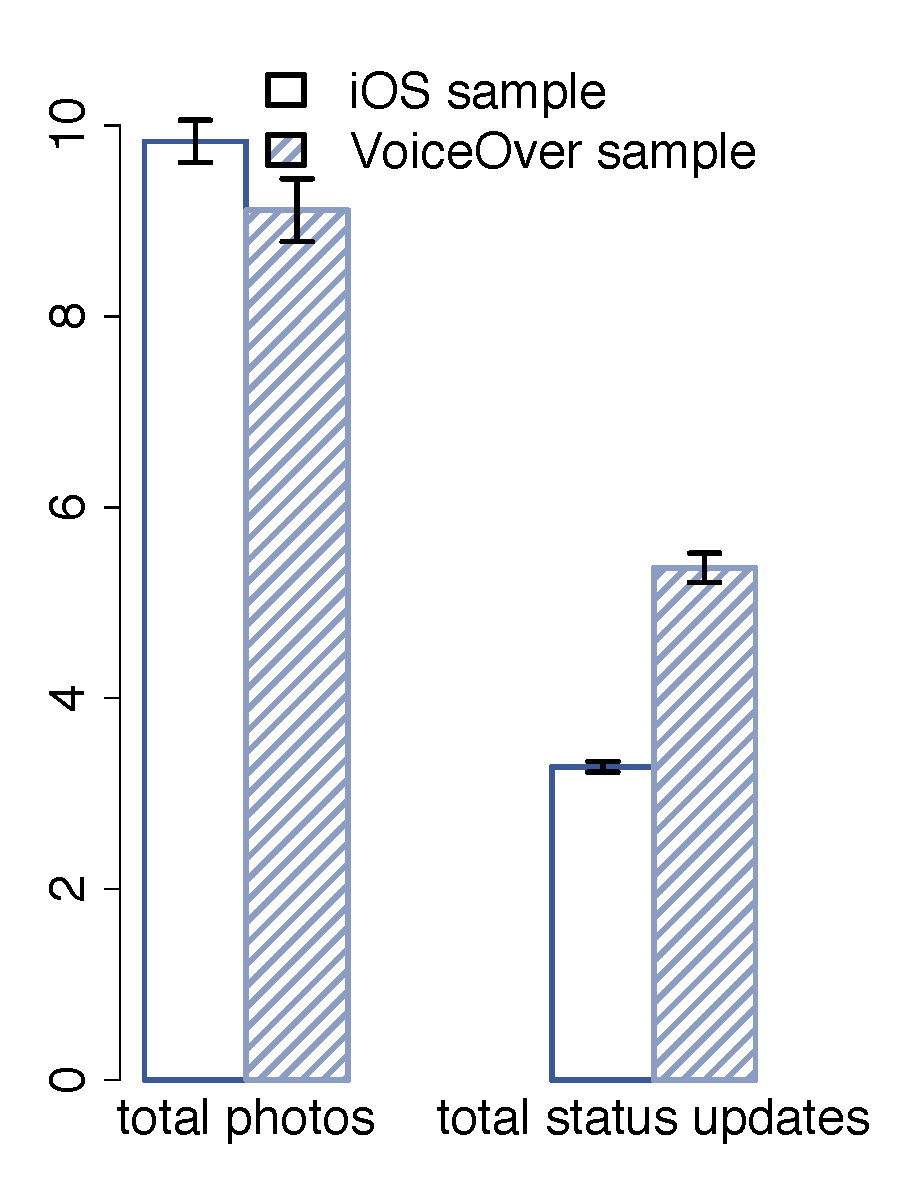
\includegraphics[width=\columnwidth]{content_produce.pdf}
    \caption{Content produced}
    \label{fig:content_produce}
 \end{subfigure}
\begin{subfigure}[b]{0.35\textwidth}
    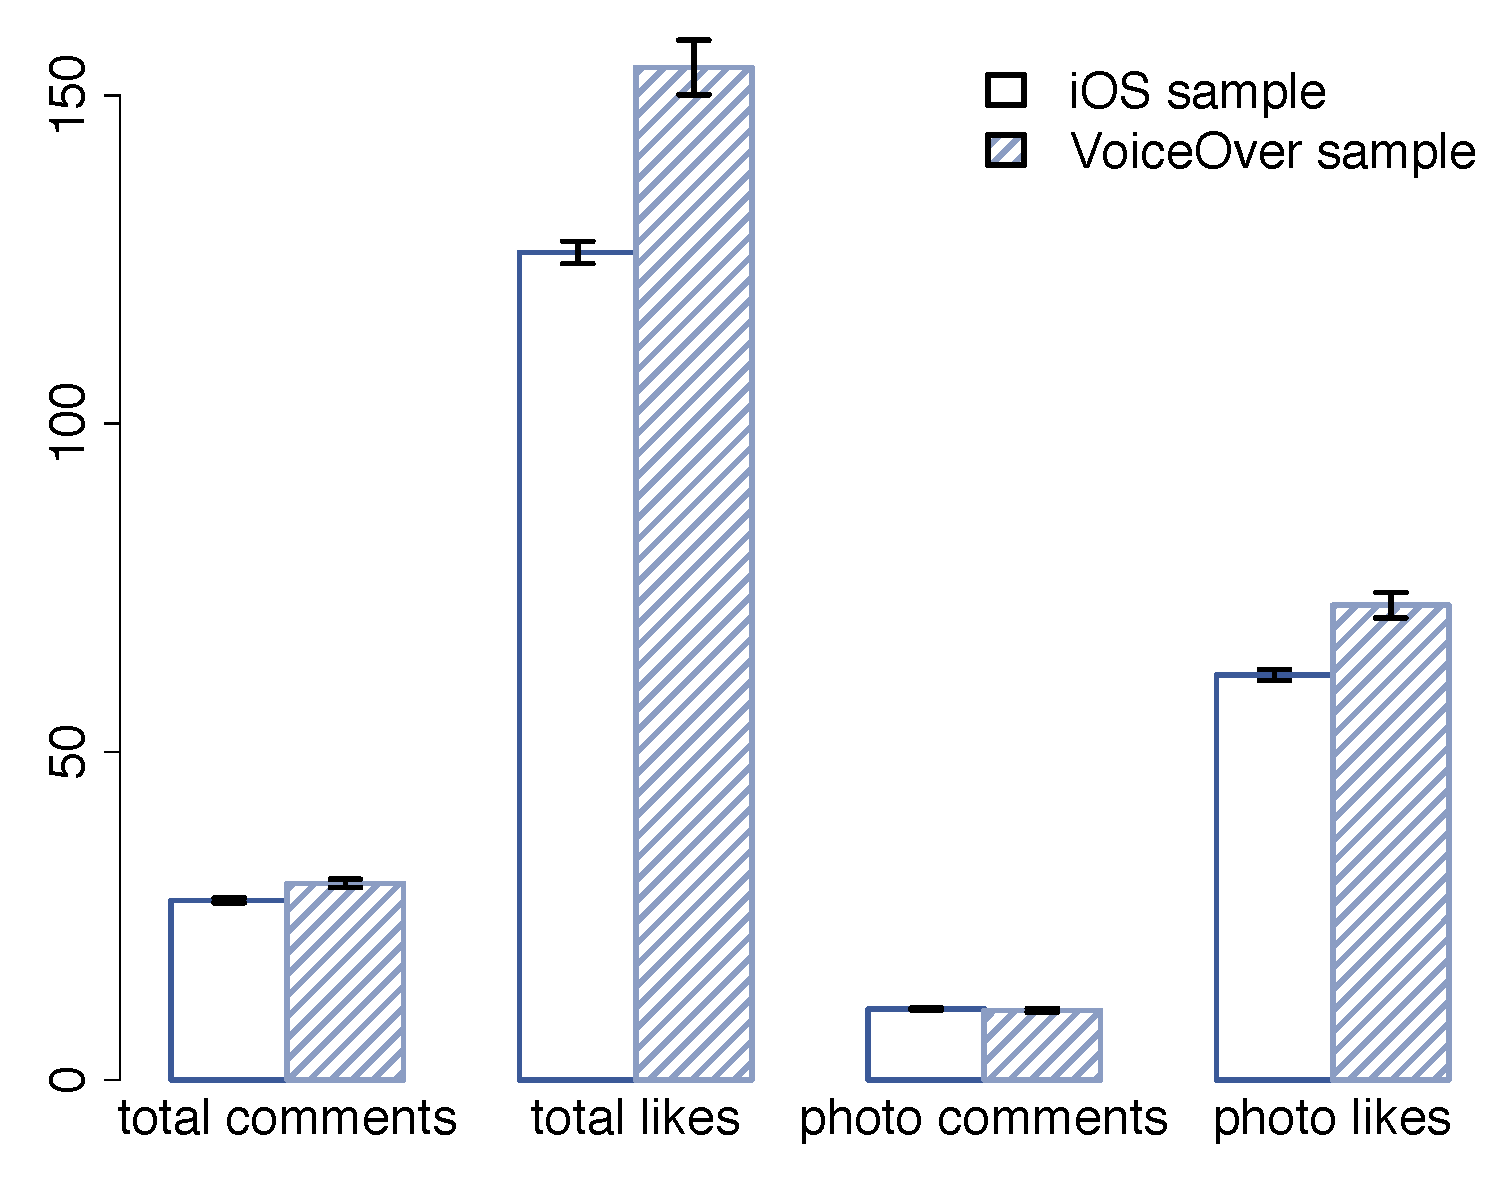
\includegraphics[width=\columnwidth]{feedback_send.pdf}
    \caption{Feedback sent}
    \label{fig:feedback_send}
 \end{subfigure}
\begin{subfigure}[b]{0.38\textwidth}
    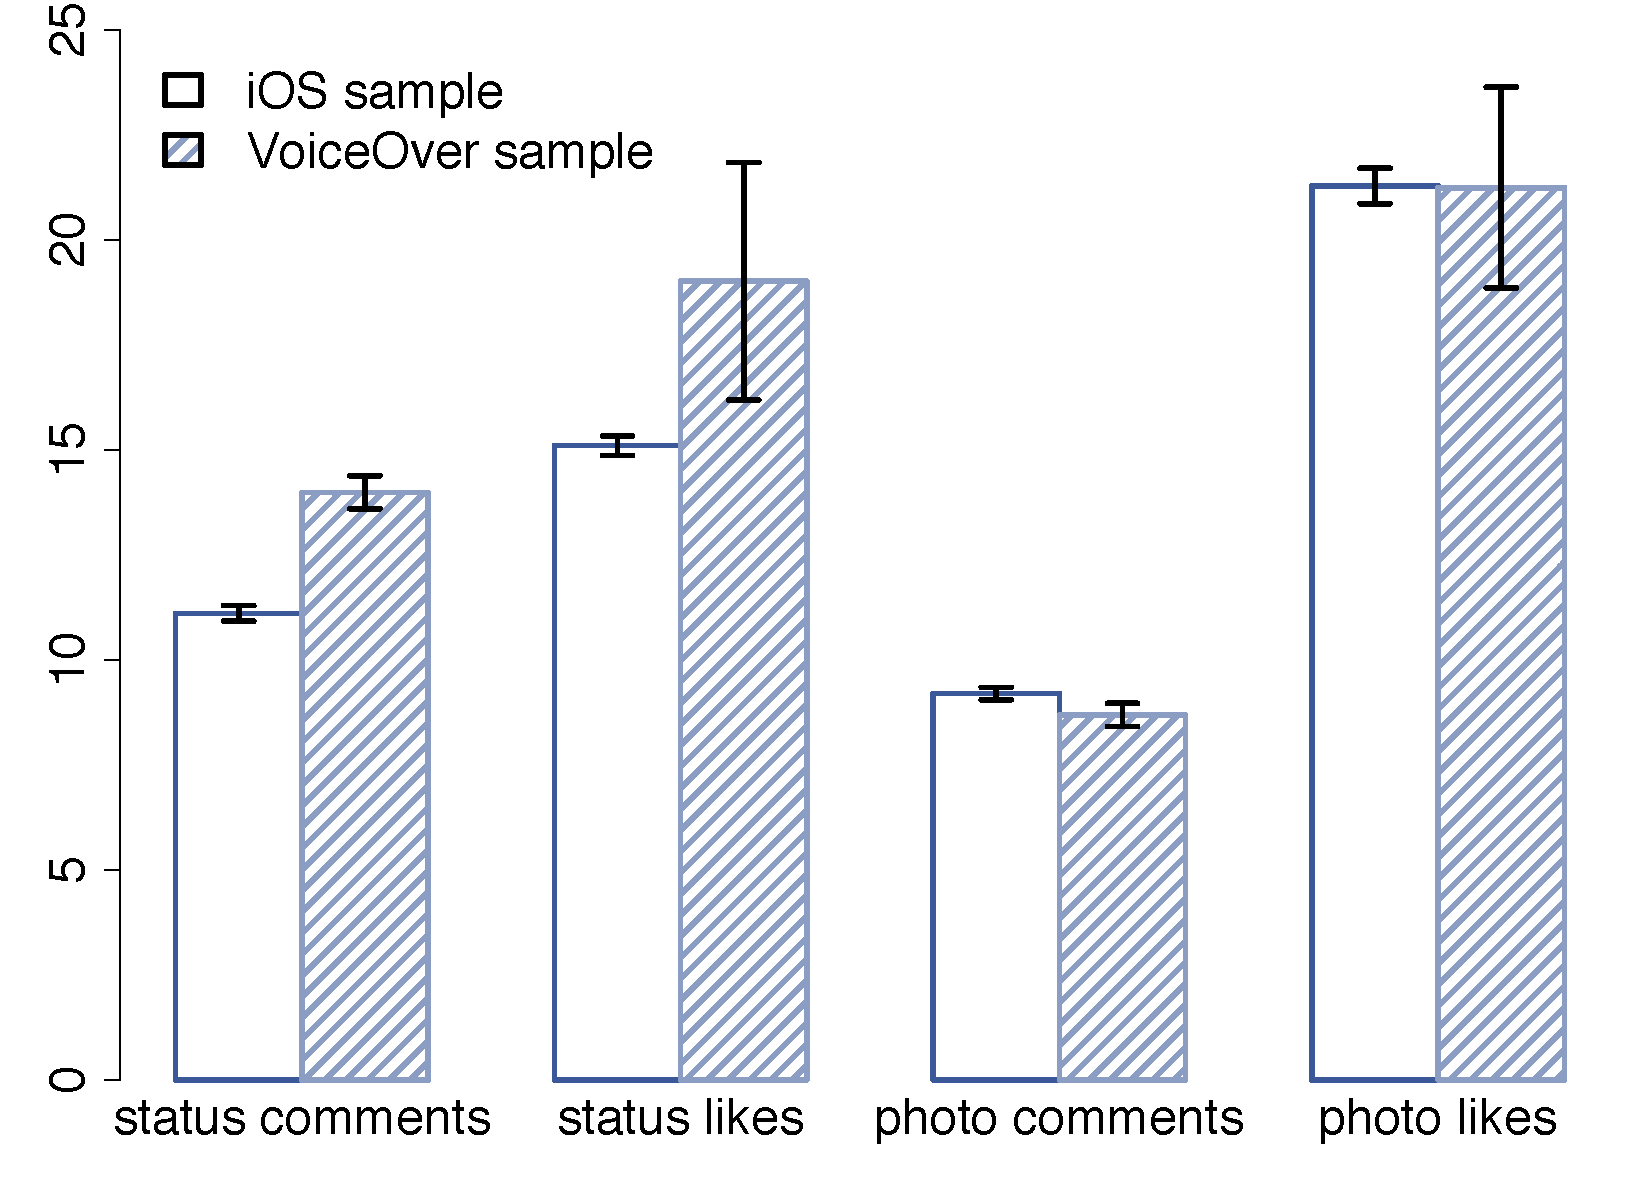
\includegraphics[width=\columnwidth]{feedback_receive.pdf}
    \caption{Feedback received}
    \label{fig:feedback_receive}
 \end{subfigure}
\caption{Per user activity over three weeks, averaged across user samples}
\label{fig:activity}
\end{figure*}


As an online social network, Facebook is most commonly used to share content (e.g., status updates, photos) and interact with content shared by friends (e.g., comments, likes).  We thus focus on the four most representative activities - status updates, photo sharing, comments, and likes - and study how visually impaired users engage with these four types of activities on Facebook. We try to understand:

\begin{itemize}
\item What do visually impaired users do on Facebook? Do they generate a different amount of content as other users?
%Whether the visually impaired users are able to engage with SNS as much as sighted users? In other words, is there any particular activity that they engage significantly more/less than sighted users?
\item How do other users interact with the visually impaired? Are they aware of the presence of visually impaired users online? Do they engage with this population, or reject them?
%\item What kind of content are shared by visually impaired users? Do they talk about their disabilities, or that is a taboo topic to them?
%Particularly, as many previous studies have emphasized the prospective that visually impaired users leverage the power of social networks to ask vision-related questions and get help ~\cite{brady2013cscw}?
\end{itemize}

To answer these two questions, we collect all the status updates, photo uploads, comments and likes by all the users in the VoiceOver sample and the iOS sample, from August 4, 2013 to August 25, 2013 (in total 3 weeks), as well as all the feedback (comment and likes) on this content recieved within a week of posting.  Then we compare the volume of content created and feedback received across the two groups. 

%the content shared by visually impaired users at such a large scale, we extract the text from status updates and photo captions, and show the most representative terms in visually impaired users status and photos.
 
% Also talk about the numbers in the figures. And label the figures better (differentiate the receive with produce)
In Figure~\ref{fig:activity}, we break down user activity into three categories: content produced, feedback sent, and feedback received, and we show each metric averaged over each user group along with error bars indicating the $95\%$ confidence interval (assuming normal distribution). For example, in Figure~\ref{fig:content_produce}, we count the total number of status updates and photo uploads in three weeks for each user, and plot the average value for users in iOS sample and VoiceOver sample. We can make two interesting observations from this plot: first, visually impaired users post many more status updates than the control group; second, although visually impaired users do upload fewer photos than users from the control group, the gap is surprisingly small - visually impaired users are producing and sharing a lot of photos on Facebook. 

Inspired by this finding, we also separate the number of comments and likes by the type of the content being responded to: photos or status updates. As shown in Figure~\ref{fig:feedback_send} and Figure~\ref{fig:feedback_receive}, compared to other users, visually impaired users:
\begin{itemize}
\item give significantly more likes in general, including more likes of photos posted by others;
\item receive more likes and comments on their status updates, but not on their photos.
%\item  although only give similar amount of comments, but receive significantly more comments on their status updates.
\end{itemize}

Overall, VoiceOver users are highly active at generating content and giving feedback to others' content on Facebook. There is no siginificant evidence that their ability to engage with the service is confined or limited compared to other users. Moreover, the visually impaired users in our sample on average receive more feedback on their status updates (and presumably more attention) from other users on Facebook. 

% link this paragraph better with the previous one
In terms of photo-related activities, VoiceOver users do upload slightly fewer photos, but they comment on as many photos as the iOS sample users, and like even more photos. However, different from the status updates, the photos uploaded by VoiceOver users do not receive more comments or likes from others compared to the photos uploaded by users in the iOS sample.

Since some previous studies suggest that crowdingsourcing, or friendsourcing vision-related questions on social networks can be a great resource for blind users \cite{brady2013cscw, brady2013chi}, we also examine the question-asking activity of visually impaired users on Facebook by looking for question marks in status updates and photo captions, a heuristic method commonly used in prior studies \cite{morris2014,paul2011}. Figure~\ref{fig:question_ask} shows the total number of questions asked in status updates and photo captions over three weeks, averaged per capita for each sample group\footnote{Here we show the raw number of questions instead of the proportion of them in status updates, because many users did not post any status updates in the entire period thus it is not clear what the proportion means in those cases. When only considering users with status updates, the median ratio of questions in status updates is $0$ for both groups.}.  Additionally, we calculate the ratio of questions in all status updates and in all photos (aggregated over each sample), and find: over all status updates posted by VoiceOver users, $17\%$ of them contain a question mark, compared to $18\%$ in the iOS sample; and for photos, only $0.4\%$ of the photos uploaded by VoiceOver users contain question marks, exactly the same fraction as in the iOS sample. Overall, we find that the question-asking behavior is rare in both populations, and asking question about photos is particularly uncommon. This result is consistent with previous findings that blind users are reluctant to ask vision questions to their social networks due to the high social cost perceived \cite{brady2013cscw}. However, when the visually impaired users do ask questions through social media, they receive significantly more response than the general population does (see Figure ~\ref{fig:question_response}). 

%\textcolor{green}{Maybe instead of the raw count, using the ratio of questions in all status updates and in all photos (aggregated over each sample). For example, over all status updates posted by VoiceOver users, $17\%$ of them containing question mark, but for iOS sample, $18.2\%$ containing question marks. And for photos, only $0.4\%$ of the photos uploaded by VoiceOver users contain question mark, and the number is exactly the same for iOS sample.}



%Reason for give more photo likes: less discrimative about photo quality? generally giving more likes
%Reason for receive less photo likes: many photos are automatic uploads, or test photos.


% When studying the amount of feedback sent by sampled users to others, we not only look at the total number of comments and likes generated by these users in the study period, but also more specially, the number of comments and likes associated with photos.

%In Figure ~\ref{fig:feedback_send}, we not noly show the average number of all comments and likes produced by users from two groups, but also the 

 %shows the average number of status updates and photo uploads in three weeks, with the error bars indicating the $95\%$ confidence level of the mean value (

%At a high-level, we see very similar level of activeness in status updates, comments, and likes. Not surprisingly,  visually impaired users do engage much less with photo-related features such as photo uploads, photos comments and likes. However, when visually impaired users do upload photos, their photos receive more attention and feedback from other users. In our content analysis, we find that question asking is quite rare in either status or photos, for both visually impaired users and sighted users, but visually impaired users do openly talk about issues related to vision disability and accessibility. Also, we are able to identify several technologies and applications besides VoiceOver (e.g., TapTapSee, tunein, peachtree audio) that are especially popular among the visually impaired users. This finding can help us not only improve the intergation of social media and these apps for a more accessible and smoother experience, but also better identify and recognize visually impaired users on the site.  

%In the rest of this section, we will present more detailed results on status updates and photo sharing.

%create, share and consume personal content (status updates, photos, etc. 

%Most representative activities.

%High level: very similar level of status updates, comments, and likes, but much less photo-related activities.

%Barplot of different activities (separate status/photos with comments and likes?)

%More specific: similar use of privacy settings;  question asking in either status or photos is low for both the blind community and the control group.


\begin{figure}
\centering
\begin{subfigure}[b]{0.23\textwidth}
    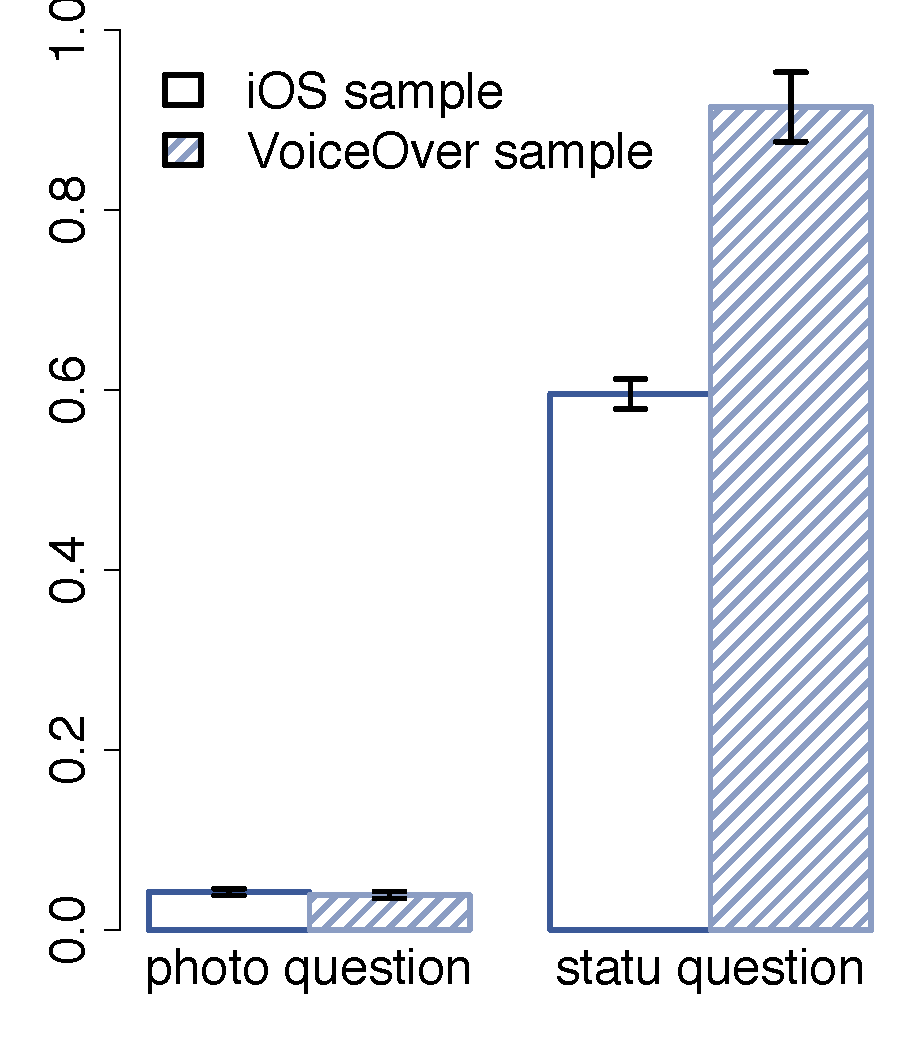
\includegraphics[width=\columnwidth]{question_ask.pdf}
    \caption{Question asking}
    \label{fig:question_ask}
 \end{subfigure}
\begin{subfigure}[b]{0.23\textwidth}
    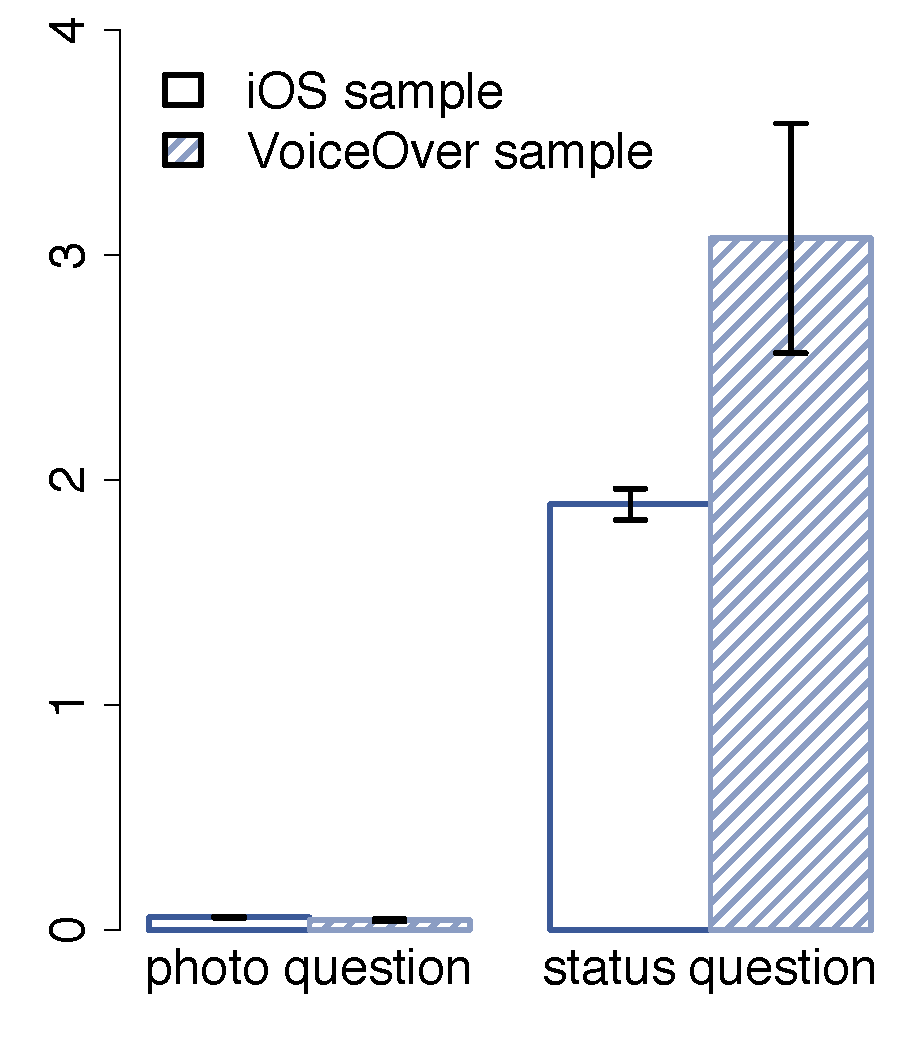
\includegraphics[width=\columnwidth]{question_response.pdf}
    \caption{Question response}
    \label{fig:question_response}
 \end{subfigure}
 \caption{Social Q\&A and response received on Facebook: (a) total number of questions asked in status updates and photo captions; (b) total number of people who respond to questions asked by sampled users.}
\label{fig:question}
\end{figure}

\section{Content Analysis}

Knowing that visually impaired users actively produce and share content on Facebook that generates feedback at higher rates than average, we would like to take a closer look at the content itself, looking for the key differences between the content shared by the visually impaired and the general population. What do visually impaired users talk about in their status updates? What kind of photos do they upload? Do they talk about their disabilities? Why do we see disproportionally more feedback on the content produced by visually impaired users?

To answer these questions, we take all the textual content in status updates and photo captions by sampled users with locale `en-US' (US English),  and apply the trend detection algorithm as described in \cite{kleinberg2004}.  Using the colletion of text produced by users in the iOS sample as a baseline, we find the most representative words used by VoiceOver users with both the absolute change metric and the probability change metric. Although the probability change metric has been most recommended and widely applied in the industry \cite{FacebookTrend}, we include the results based on the absolute change metric because it favors words with higher frequencies \cite{kleinberg2004}. Thus, it can offer a better sense about the prevelance of those selected words and prevent our results from being dominated by a small set of highly distinctive (but relatively infrequent) words. 

As we have seen in the previous section, people respond more to status updates than to the photos by VoiceOver users (see Figure~\ref{fig:feedback_receive}). To better understand the differece in the nature of these two types of content, we separate the text in status updates from that in photo captions and run the trending term detection algorithm independently on each corpus. 

At a high level, we find that visually impaired users do openly talk about issues related to vision disability and accessibility. Also, we are able to identify several technologies and applications besides VoiceOver (e.g., TapTapSee, tunein, peachtree audio) that are especially popular among the visually impaired users. This finding can help us not only improve the intergation of social media and these apps for a more accessible and smoother experience, but also better identify and recognize visually impaired users on the site.  

In the rest of this section, we will present a more detailed analysis on status updates and photo captions.


\subsection{Status Updates}

Our method for identifying the most representative words is a direct application of the two-point trends detection algorithm as described in~\cite{kleinberg2004}: using the status updates of iOS sample users as text from the first time period and the status updates of VoiceOver sample users as text from the second time period, we want to find the words with the most significance ``rising'' patterns from the first time period to the second time period. To measure the signficance of the change, we use normalized absolute change and probability change metrics defined as below:
 
Let $n_0$ and $n_1$ denote the total number of token in the text from the first and second time periods respectively, and $f_0(w)$ and $f_1(w)$ denote the frequency of the word $w$ in the first and second time periods respectively, we define the \textbf{normalized absolute change} for word $w$ as 
\begin{equation}
f_1(w)(n_0/n_1)-f_0(w),
\end{equation}
 and the \textbf{probability change} as 
\begin{equation}
{n_1 \choose f_1(w)}p_0(w)^{f_1(w)}(1-p_0(w))^{(n_1-f_1(w))},
\end{equation}
here $p_0(w)=f_0(w)/n_0$, $p_1(w)=f_1(w)/n_1$.

When adopting the algorithm to our dataset, we first filter out all terms with length less than 4 (mostly numbers and stop words). To further reduce the noise in our data, we also filter out the terms that appear less than 10 times in the VoiceOver sample, and less than 30 times in the iOS sample (since iOS sample has 3 times more people than the VoiceOver sample). We then normalize the language use across users by only counting each word at most once per user, which effectively reduce the algorithm's bias towards words used by users who post long, repetitive status updates (e.g., pet's names). The top 10 words selected by these two metrics from all status updates in the VoiceOver user sample are shown in Table~\ref{tab:status_top_words} (all text is converted to lowercase).

\begin{table}
  \centering
  \begin{tabular}{c|c}
    \hline
      \tabhead{Abs. change} & \tabhead{Prob. change} \\
    \hline
  blind & blind \\
  braille & braille \\
  guide & sighted \\
  accessible & blindness \\
  sighted & goalball \\
  cane & voiceover \\
  audio & paratransit \\
  blindness & inaccessible \\
  impaired & accessible \\
  visually & impairment \\
  \hline
  \end{tabular}
  \caption{Top 10 most representative words in the status updates of VoiceOver users. }
  \label{tab:status_top_words}
\end{table}

It is striking to see that the top 10 words by both metrics are all related to vision impairement\footnote{Goalball is a sport developed specifically for blind atheletes}: compared to other iPhone users, VoiceOver users on Facebook are more likely to discuss vision impairment and accessibility issues found in both the physical world and on the Internet. The highly characteristic content generated by visually impaired users distinguishes them from other social media users, potentially allowing for the automatic detection of users with vision disability by their language use. Meanwhile, the uniqueness in the status updates of visually impaired users could also contribute to the higher volume of feedback from other users, as being perceived as more interesting/meaningful/important.



\subsection{Photo Sharing}
Knowing that visually impaired users post almost as many photos as the average iOS user, we want to assess the content of these photos, and understand whether visually impaired users upload photos that are as characteristic as their status updates. And if yes, why do visually impaired users' photos not receive as much feedback from others as their status updates do?

We apply the same method as presented above, this time with the collection of text from photo caption. In Table~\ref{tab:photo_top_words}, we show the top 10 most representative words that describe VoiceOver users' photo uploads.

\begin{table}
  \centering
  \begin{tabular}{c|c}
    \hline
%    \multicolumn{1}{|p{0.1\columnwidth}|}{\centering\tabhead{Rank}} &
 %   \multicolumn{1}{|p{0.2\columnwidth}|}{\centering\tabhead{Caption --- pre-2002}} &
  % \multicolumn{1}{|p{0.2\columnwidth}|}{\centering\tabhead{Caption --- 2003 and afterwards}} \\
   \tabhead{Abs. change} & \tabhead{Prob. change} \\
    \hline
  tunein & peachtree \\
  radio & tun.in/se8qe \\
  listening & hatchi \\
  peachtree & facebook.com/hatchiapp \\
  tun.in/se8qe & \#dailyquote \\
  hatchi & taptapsee \\
  facebook.com/hatchiapp & solara \\
  \#dailyquote & itunes.com/apps/esperlabsllc/solara \\
  taptapsee & navy/gold \\
   bit.ly/11j2rfj & tunein \\
  \hline
  \end{tabular}
  \caption{Top 10 most representative words in the photo captions by VoiceOver users. }
  \label{tab:photo_top_words}
\end{table}

At a first glance, the buzzwords picked from photo captions do not appear to be as relevant to vision disability as the words from status updates are. We see some words related to listening to radio (e.g. ``listening'', ``radio'), which makes sense since visually impaired users do listen to radio programs much more than sighted users. Following this clue, we realize that most of the words shown in Table~\ref{tab:photo_top_words} are related to \emph{specific activities or applications visually impaired users engage with} online or with their mobile phones. For example, \textit{tunein} is probably from the product named ``TuneIn Radio'', one of the largest mobile applications for online radio (including radio stations and podcasts) \cite{tunein_wiki}. And \textit{peachtree} \footnote{\url{http://tunein.com/radio/Peachtree-Radio-FM-s198932/}} is a popular radio station on TuneIn Radio. Photo captions containing ``peachtree'' are mostly formulaic, such as: ``I am listening to Livin' On A Prayer by Bon Jovi on WICS Radio America with TuneIn Radio \url{http://tun.in/seXtz}'' (quote is taken from publicly shared status updates). In the end, we would like to highlight a very popular photography application for iPhone users with vision impairement - \textit{TapTapSee}\footnote{\url{http://www.taptapseeapp.com/}}. As described in the top customer review in iTunes AppStore\footnote{\url{https://itunes.apple.com/us/app/taptapsee-blind-visually-impaired/id567635020?mt=8}}: ``It is a camera [app] that when a picture is taken will give back a verbal description of what is seen. I use it to detect colors in order to cord Nate [sic] my wardrobe. It is one of the most helpful apps that I have on my iPhone.'' Hundreds of VoiceOver users in our sample have taken photos with this application and uploaded these photos to Facebook with captions like ``I discovered this was a `Nature Valley Oats N Honey Bar And Ceramic Mug On Table` with TapTapSee'' and ``I discovered this was a `Coca Cola Can` with TapTapSee'' (both quotes are taken from publicly shared photos on Facebook). 

The top keywords from photo captions suggest that many of the photos uploaded by visually impaired users are automatically created and captioned by other apps instead of the users themselves. As a result, these photos may be viewed by others as less authentic or spammy, and thus attract less feedback than the status updates do. Meanwhile, with the popularity of photo Q\&A systems such as TapTapSee and VizWiz \cite{jayant2011}, more and more blind users can get satisfactory answers to vision question without paying the high social cost of directly polling their friends in social networks\cite{brady2013cscw}. 

To summarize our content analysis, we find that visually impaired users openly talk about their experiences and issues with vision disability and web accessibility. Their stories and concerns are well received and elicit active response from other users of the social network. Our trend detection algorithm is able to identify the most characteristic words and applications used by the visually impaired users, showing great potential toward a better profiling scheme for this specific population.

 
%Many photos are a by-product of other activities such as radio and games and photography apps, and are not posted specifically for sharing the experience. Many of them can have lower than average quality.  Reasons for not getting more comments and likes (taptapsee photos are already the answer to users' questions).

% more examples:

%"I discovered this was a 'Woman Wearing Black Fur Hat ' with TapTapSee"
%"I discovered this was a 'Golden Wonder Cheese & Onion Chips' with TapTapSee"
%"I discovered this was a 'due persone che abbracciano' with TapTapSee"

%"I discovered this was a 'rosto humano' with TapTapSee"
%"I discovered this was a 'Flatscreen Television In Living Room' with TapTapSee"



% Should we also talk about the hashtag usage?

%Findings: 
%\begin{itemize}
%\item Blind users openly talk about their experience and issues with web accessibility - big concerns, call for more attention and improvement.
%\item We can identify the most popular applications and activities (online radio, peachtree) for the blind population - possibly intergrate them better with social media sites.
%\end{itemize}



\section{Network Structure}

In previous sections, we found that visually impaired users are actively engaging with their social networks, talking about their conditions and concerns openly, and receiving more feedback from other users. But how much of these observations can be explained by the structural properties of visually impaired users' social networks? For example, as previous study showed that users with more diverse and sparser friendship network perform more self-censoring on Facebook \cite{das2013}, can the openness we observe in vision-imparied users be a result of their social networks being denser than average? On the other hand, the reason that visually impaired users receive more comments and likes may simply be that they have more friends (and thus a bigger audience) than an average user.

To answer these questions, we will study in-depth the structural properties of the social networks around visually impaired users, focusing on the network size, density, and the interconnectivy among visually impaired users. 

%High unemployment rate for blind population, as a result, more limited social contact and more homogenous social networks.

%Hypothesis: blind users have smaller but denser social networks?


\subsection{Network Size}

Previous work has suggested that blind users have smaller social networks than average \cite{brady2013cscw}. In our data, the median friend count is $208$ for users in the VoiceOver sample, and $242$ for the iOS sample. The mean value for VoiceOver sample is $339.9$, and for iOS sample is $367.5$. Although all these numbers are much higher than reported~\cite{brady2013cscw}, a student t-test comparing the mean friend count across these two samples gives $p<2.2e-16$, showing high confidence that the average network size is greater in the general iOS sample than in the VoiceOver sample. 

Also, as the VoiceOver sample may contain users with different levels of vision impairement, we also extract the set of users who mentioned ``TapTapSee'' in their status updates or photos, and use them as a confident representation of blind (or near-blind) users. We denote this set of users as the \emph{TapTapSee sample}. We then take the median and mean friend count for users in the TapTapSee sample, which are $161$ and $222.4$ respectively. These numbers are even lower than what we get in the VoiceOver sample, although still higher than the average~\cite{ugander2011}.


It seems that visually impaired users do on average have smaller social networks, as comparing to other users. However, since it takes much longer to accumulate friends than to generate content, and newer users will in general have fewer friends than users that have been on Faecbook longer, we want to further test to what extent the difference in friend count between these two groups can be explained by the difference in Facebook tenure.  As the devolopment of web accessibility has progressed so rapidly in the past few years, only recently have visually impaired users become able to use social networking services as easily as other users \cite{wentz2011}. In fact, when comparing the ``Facebook age'' (number of days since a user joined Facebook) across these two samples, we find that VoiceOver users are in general newer to Facebook than the average iOS users: the median Facebook age for VoiceOver sample is $38$ months whereas for iOS sample is $46$ months (t-test on sample mean gives  a $p$-value less than $2.2e-16$). To illustrate how friend count changes with Facebook age, we plot the median friend count for users who joined Facebook in the same month (see Figure~\ref{fig:friendcount_facebookage}). Our result shows that the gap in the network size of these two populations has been descreasing in recent years. Especially, when we control for Facebook age, new Facebook users (i.e., people who joined in the past 2 to 3 years) seem to have similar network size whether they are part of the VoiceOver or iOS group.
% TODO: Are TapTapSee users newer still than VoiceOver users?

%visually impaired users seem to have similar network size as the average user, especially,  for everyone who are relatively new to Facebook (joined in the past 2 to 3 years). 
 
% TODO: tweak this figure more.
\begin{figure}[htb]
\centering
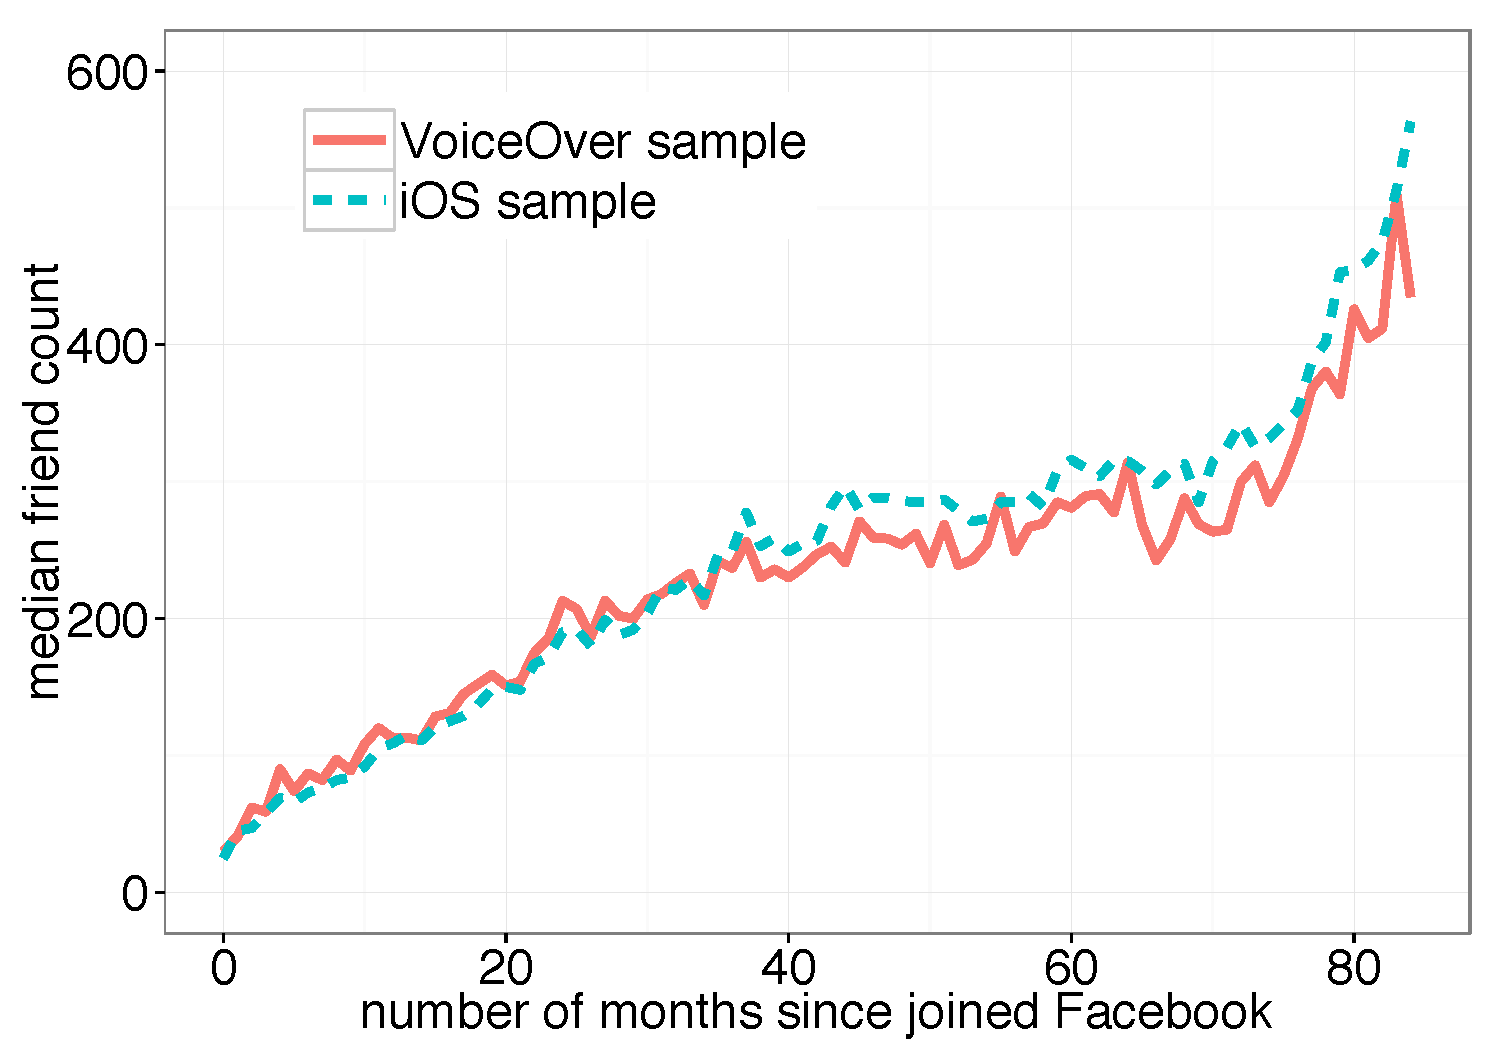
\includegraphics[width=0.9\columnwidth]{friendcount_facebookage.pdf}
\caption{Network size as function of Facebook age.}
\label{fig:friendcount_facebookage}
\end{figure}

\subsection{Network Density}

Another hypothesis we want to test is that visually impaired users have more homogenous, and thus denser social networks. Previous research showed that blind users on Facebook have their social networks comprised primarily of friends, family and colleagus (in total over $95\%$ of all Facebook friends) \cite{brady2013cscw}. Also, our earlier analysis demonstrated that visiually impaired users engage with Facebook actively, and receive more feedback on their content than other users do. As a result, we expect that the friends of a visually impaired user are more likely to also be friend with each other (maybe through both engaging with the content generated by their visually impaired friend), forming a more intimate, tightly connected social network. To measure the connectedness of a user's social network, we define the ego graph clustering coefficient of a user $u_i$ as:
\begin{equation}
C_i=\frac{\text{number of edges between } u_i\text{'s friends}}{n_i\times(n_i-1)/2}
\end{equation}
Here $n_i$ is the number of friends $u_i$ has.

The greater $C_i$ is, the denser user $u_i$'s social network is. $C_i$ is $0$ when none of $u_i$'s friends connects to each other, and is $1$ when $u_i$'s friends form in a fully connected clique. As clustering coefficient is in general very sensitive to the size of the ego graph ($n_i$) - it is much easier for small graphs to have higher clustering coefficient than big ones - we control for the size of individual's ego graph and plot the value of clustering coefficient as a function of ego graph size in Figure~\ref{fig:friendcount_density}. At a high level, the curves for the VoiceOver sample and the iOS sample are almost identical, showing no evidence that visually impaired users have denser social networks than the general population.
However, the result is reversed when comparing the iOS sample with the TapTapSee sample, especially when the number of friends is small (less than 50), suggesting that most TapTapSee users in our sample have very small but extremely dense social networks on Facebook\footnote{Note that as friend count increases, the data get very sparse for TapTapSee sample, which is consistent with previous result that TapTapSee users in our sample in general have smaller social networks than the others. We still show the curve just to be consistent with the other samples.}. 


% Figure ~\ref{fig:clustering_coefficient} shows the empirical CDF curves for the values of ego graph clustering coefficient in different samples. At a high level, the result is consistent with our hypothesis: although very similar, VoiceOver users do have overall slightly smaller ego graph clustering coefficient than the general iOS sample. However, the result is reversed when comparing the iOS sample with the TapTapSee sample: TapTapSee users seem to have denser social networks than the control group.  

% Shaomei: replace this plot with the one below per Lada's suggestion.

%\begin{figure}[htb]
%\centering
%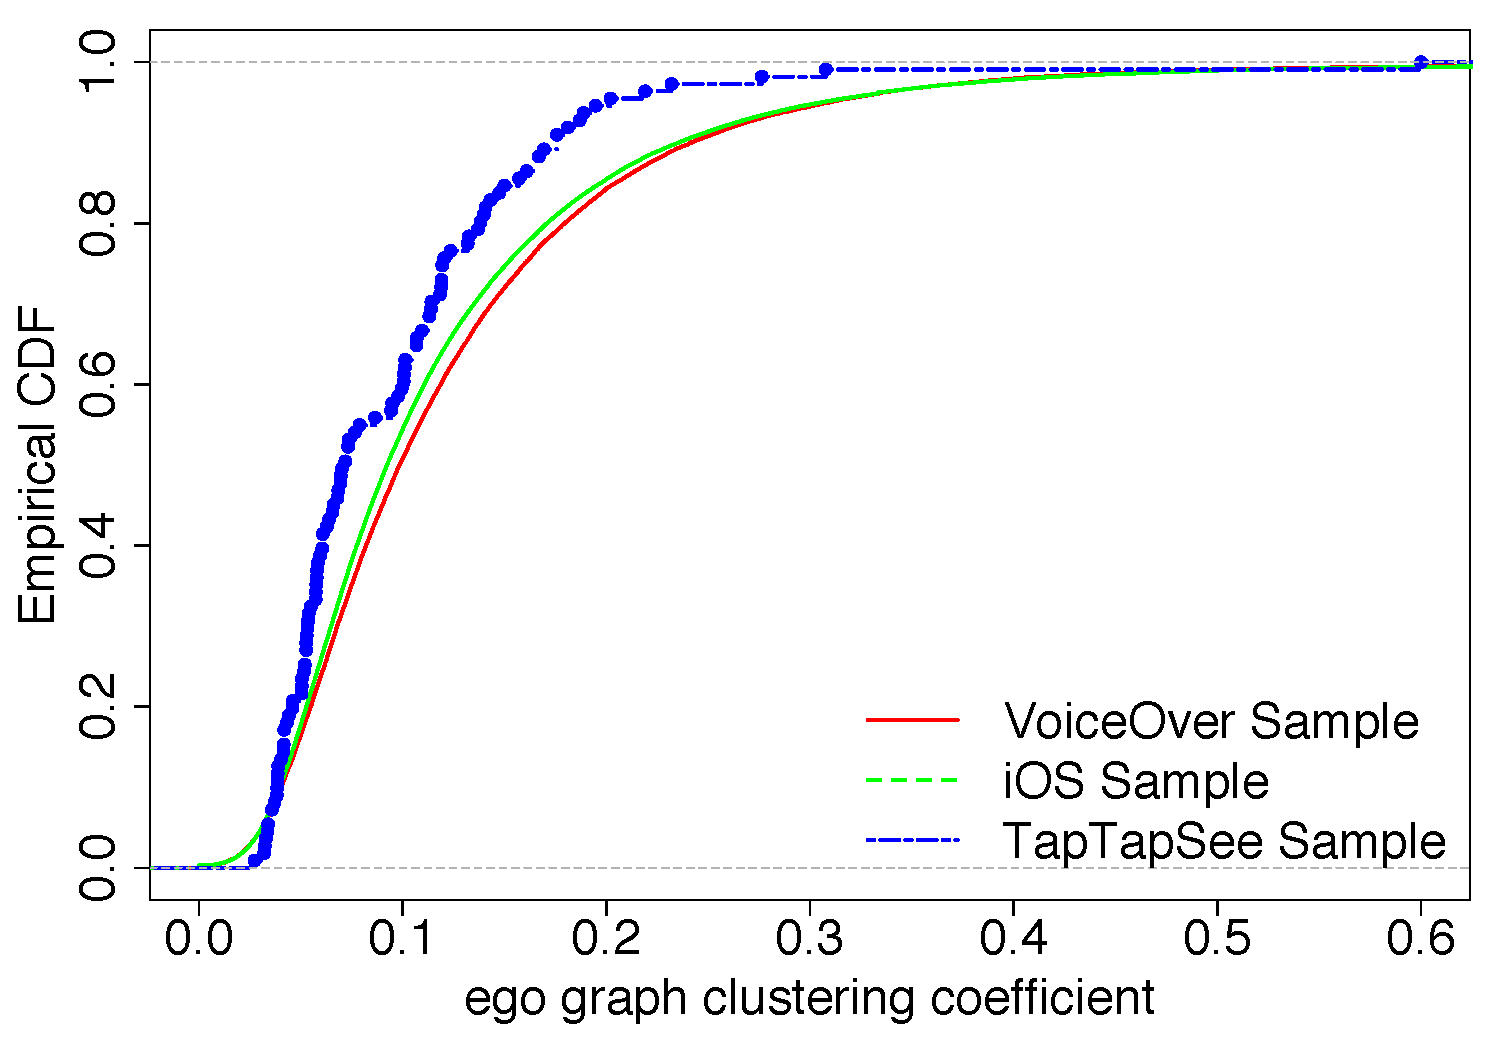
\includegraphics[width=0.9\columnwidth]{cluster_coefficient.pdf}
%\caption{Distribution of ego graph clustering coefficient }
%\label{fig:clustering_coefficient}
%\end{figure}

\begin{figure}[htb]
\centering
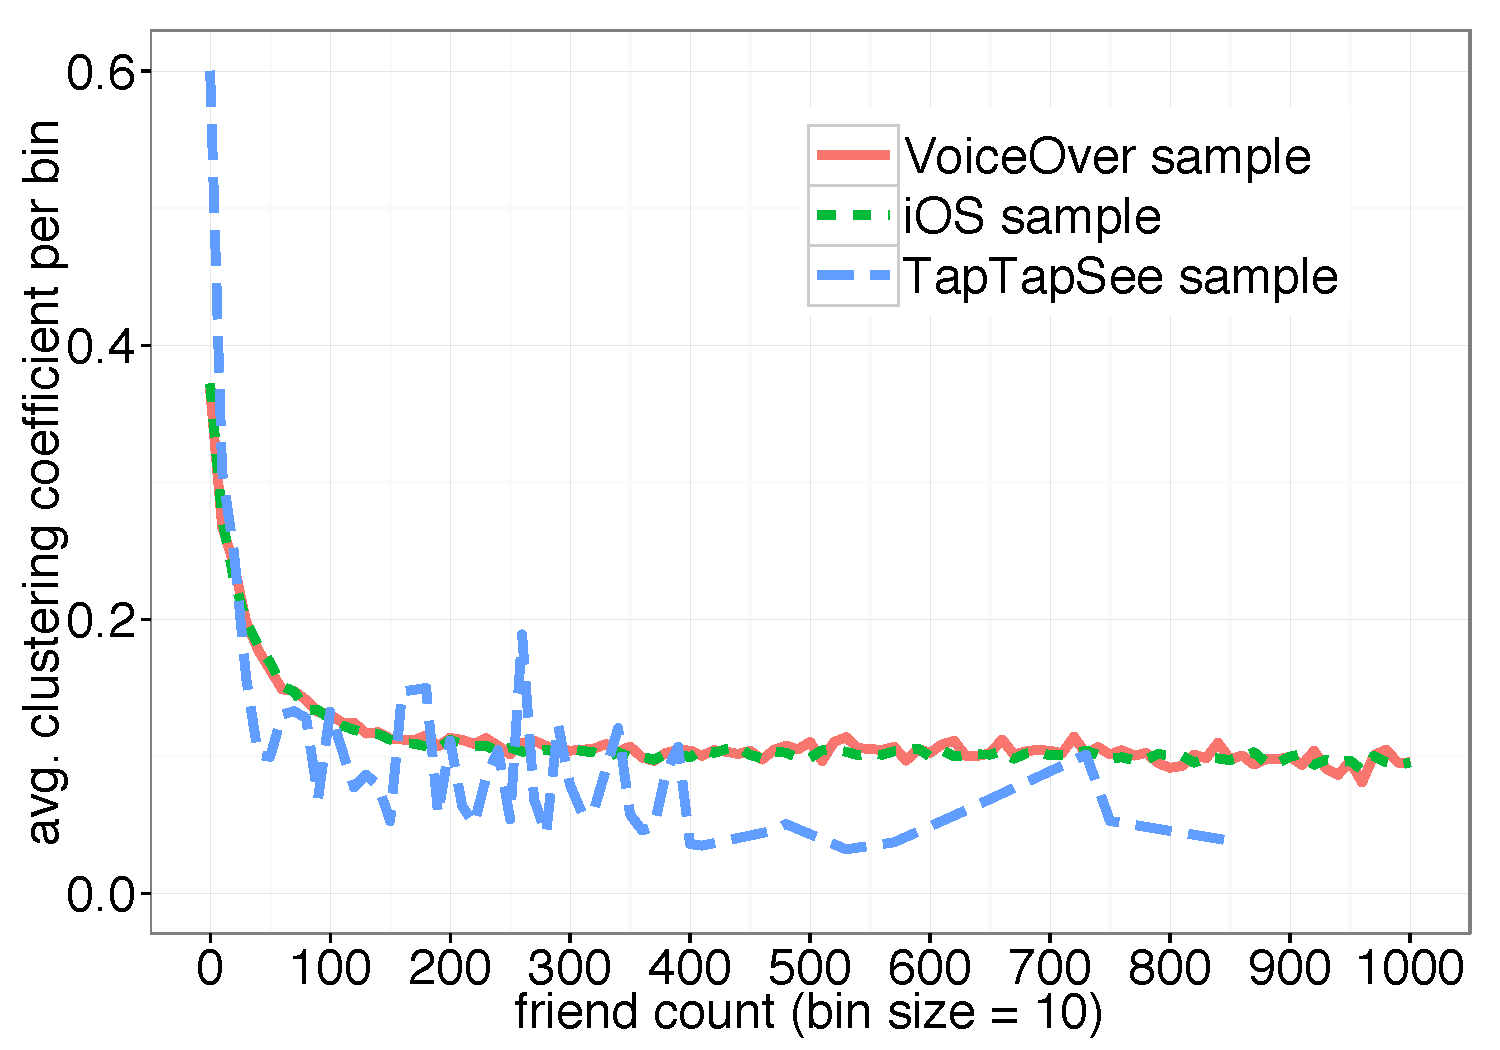
\includegraphics[width=0.9\columnwidth]{friendcount_clustering_coefficient.pdf}
\caption{Ego graph clustering coefficient as function of ego graph size}
\label{fig:friendcount_density}
\end{figure}


We can also quantify the homogeneity of a user's social network by the number of distinct social communities among his/her friends. We use the algorithm as presented in \cite{ugander2011} to detect and identify communities in each user's ego network, and show the distribution of community count across users in three samples in Figure~\ref{fig:community_count}. As Figure~\ref{fig:community_count} shows, the level of diversity in personal social networks is almost identical for users from the VoiceOver sample and users from the iOS sample, with about half of the sample having only one community, and almost $90\%$ of the sample having no more than 3 communities. Meanwhile, users from the TapTapSee sample do seem less likely to have just one community. Overall, our result confirms that most visually impaired users have closely connected social networks with a few communities (presumably formed by friends, family and colleagues), but this is also true for other users on Facebook! We do not find visually impaired users to have denser than average networks over all.

\begin{figure}[htb]
\centering
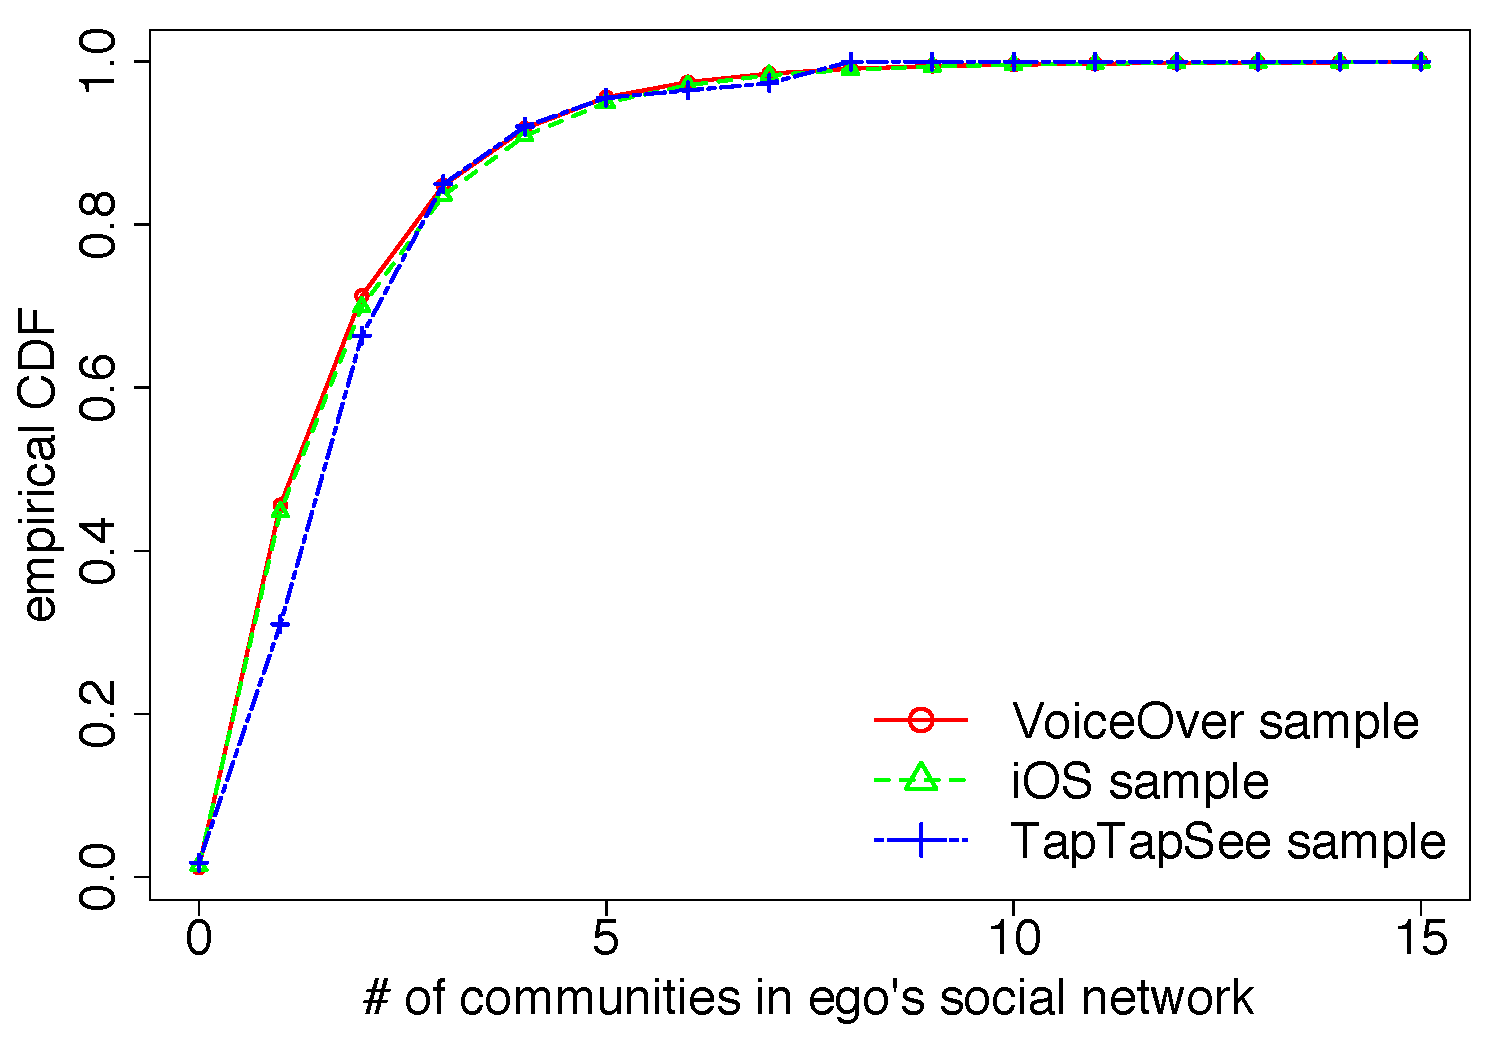
\includegraphics[width=0.9\columnwidth]{community_count.pdf}
\caption{Distribution of number of communities in a user's social network }
\label{fig:community_count}
\end{figure}

\subsection{Interconnectivity among Visually Impaired Users}
The last question we want to ask about the network structure of visually impaired users is about the interconnectivity among them: are visually impaired users more likely to be friend with other visually impaired users? Classic homophily theory would say ``yes'', however, given the fact that vision impaired users have relatively fewer friends, they are statistically less likely to have friends with any specific trait than people from the general iOS sample.

Our result supports the homophily hypothesis that visually impaired users are more likely to friend other visually impaired users. Figure~\ref{fig:interconnectivity} shows the distribution of the count of friends who are themselves VoiceOver users. Here, we can see a clear distinction between the CDF curves for these two groups: while there are less than $2\%$ of users in the iOS sample who have at least one friend in the VoiceOver sample, there are over $20\%$ of the users in the VoiceOver sample with at least one friend who is also in the sample, and around $10\%$ of the VoiceOver sample having more than 10 friends using VoiceOver as well.
 
Such signficant interconnectivity among visually impaired users would potentially introduce structural clustering of them on the Facebook network, which may eventually lead to self-organized communities of visually impaired users. This might be a factor that contributes to the charactristics of content produced and shared by visually impaired users. The structure clustering can also be very helpful when trying to auto-detect the presence of visually impaired users.



\begin{figure}[htb]
\centering
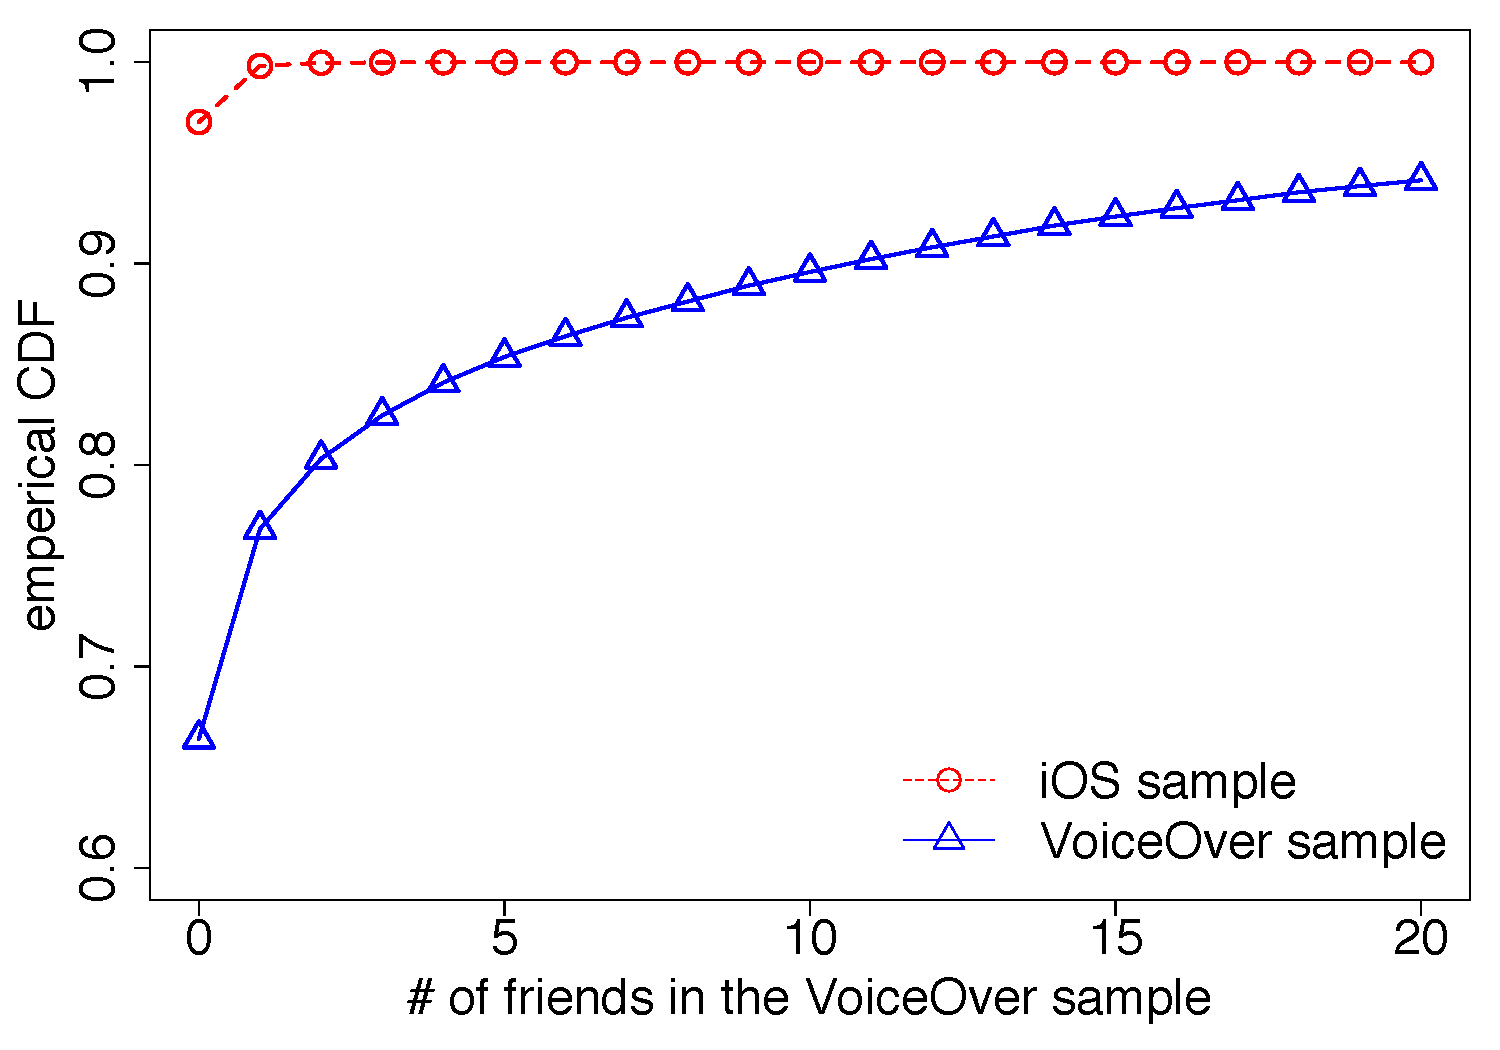
\includegraphics[width=0.9\columnwidth]{interconnectivity.pdf}
\caption{Distribution of the number of friends in VoiceOver sample}
\label{fig:interconnectivity}
\end{figure}



%\section{Disucssion}




\section{Conclusion}


%Big data enthonography: the emergence of some patterns that might not be present or observed in small-scale interviews.

% Through content analysis on the status updates and photos by sampled users, we find  that visually impaired users openly tallk about their experience and isssues with vision disability on Facebook, and have highly characteristic language and technology usage.  We also study the structural properties of vision impaired users' social networks on Facebook, hypothesizing that  visually impaired users have smaller but denser social networks. 


%Meanwhile, the developent of blind photography applications has enabled visually impaired users to take and share photos on social media.  more and more visually impaired users can share photos in social media,  

%perform as much status updates, comments, and likes as sighted users, while engage much less with photo-related featuers.  

%We find that, although technology has enabled visually impaired people to take photos and identify certain objects in digital images, the usage of photo-related features are much lower than sighted users.  However, for 



In this paper, we describe a few findings on how visually impaired users engage with online social networks, more specifically Facebook. 

We find that visually impaired users engage actively with the major social activities on Facebook (status updates, comments, and likes) just like the general population, including photo-related features (e.g., photo comments and likes). On the other hand, when visually impaired users produce and share personal content such as status updates, they receive much more feedback (i.e., comments and likes) from others than the average. These findings suggest the utility of Facebook as a platform for visually impaired users to openly share their experience, voice their concerns, and as a channel to receive attention and support from others.

We also study the content generated by visually impaired users, by running the trend detection algorithm on the text from their status updates and photo captions. We find highly characteristic keywords in visually impaired users' content: the most representative words in visually impaired users' status updates are all related to vision disability, while many of the photos are associated with (and perhaps auto uploaded by) popular applications  visually impaired users engage with (e.g. online radio, photography app). Our content analysis reveals distinctive features of the language and the activities of visually impaired users online, paving the way for devoloping machine-learning models to recognize visually impaired users beyond the population of iPhone/VoiceOver users. 

In the end, we study the structural properties of vision impaired users' social networks on Facebook, testing the hypothesis that  visually impaired users have smaller but denser social networks. We do find evidence supporting the first part of this hypothesis at a high level, however, we also notice that the difference in network size between these two groups has been diminishing over time, demonstrating our progress towards an increasingly equal and accessible online environment. We do not see clear differences in terms of the density of the network, but see a significant amount of network clustering among visually impaired users: they are much more likely to have friends who are also visually impaired. 

By analyzing the activities of visually impaired users on Facebook at a unprecedently large scale, we are able to uncover high-level patterns in the behavior and language usage of visually impaired users, which might not be present or observed at a small-scale.  However, to better explain the patterns we discovered and understand what they mean to the experience of visually impaired users on online social networks, we would need in-depth insights from qualitative studies. Also, our study has been confined to a very specific subset of visually impaired users online and in the world. In the future, we would like to apply our knowledge on the behavior and language characteristics of visually impaired users and expand our study to a more general population of visually impaired users online. As one of the first big-data studies of how visually impaired users engage with Facebook, we hope to bring more attention to the visually impaired population online and invite more research efforts to understand and address their needs. 


%But we do see a network clustering effect: visually impaired users are much more likely to have friends who are also visually impaired.

%the ego graph of vision-imparied users, and find no strong evidence that visually impaired users have smaller, or denser personal social networks, as compared to the general population.

%We also study the activities of visually impaired users on Facebook. By comparing the most common activities of vision-imparied and random-sampled users,  we find that random-sampled users engaged much more with photo-related activities, whereas vision-imparied users give and receive more positive feedback, and generate more status updates. 

%We then study the content of the status updates by visually impaired users, to understand what they share and what their concerns are. We find that, comparing to random sampled users, vision-imparied users use much less hash tags and special characters such as emoticons. 

%We also study the textual content generated by 





% Test the hypothesis that visually impaired people have smaller and denser social networks.
%Future work is to conduct qualitative study.


\section{Acknowledgments}
There are many people we want to thank. But we have to omit this section for the blind-review. 

% Balancing columns in a ref list is a bit of a pain because you
% either use a hack like flushend or balance, or manually insert
% a column break.  http://www.tex.ac.uk/cgi-bin/texfaq2html?label=balance
% multicols doesn't work because we're already in two-column mode,
% and flushend isn't awesome, so I choose balance.  See this
% for more info: http://cs.brown.edu/system/software/latex/doc/balance.pdf
%
% Note that in a perfect world balance wants to be in the first
% column of the last page.
%
% If balance doesn't work for you, you can remove that and
% hard-code a column break into the bbl file right before you
% submit:
%
% http://stackoverflow.com/questions/2149854/how-to-manually-equalize-columns-
% in-an-ieee-paper-if-using-bibtex
%
% Or, just remove \balance and give up on balancing the last page.
%
\balance


\bibliographystyle{acm-sigchi}
\bibliography{accessibility}
\end{document}
